\NewChapter{娱乐至死}
%%% See Preamble for an explanation of both of these %%%

\quote{人类无声无息地成为娱乐的附庸,毫无怨言,甚至心甘情愿,其结果是我们成了一个娱乐至死的物种。}{尼尔·波兹曼}



“娱乐至死”是尼尔·波兹曼在同名书中所说的一句名言。他认为,现代娱乐已经达到了一种“至死”的状态,使我们的思维变得肤浅、表面化,甚至忽视了我们作为人类的本质需求。这句名言广泛应用于文化和娱乐领域,形容了娱乐圈为了名誉和金钱不择手段的厮杀。而就在今晚的百老汇大剧院,一场充满杀机的戏剧即将上演!你和你的对手为争夺百老汇大剧院头牌而展开激烈的斗争。黑暗的舞台上聚光灯不时闪耀,尽一切手段,尽可能暴露在聚光灯下,成为观众的焦点吧!


\section{创作背景}
游戏创作于2022年11月,是清华大学互动媒体设计与技术专业开设的游戏引擎课课程大作业。作业要求两人一组,开发一款基于Unity引擎的3D游戏。而游戏主题采取随机抽签的模式,每一组同学要提交一个副词和一个动词进入抽奖池,再随机抽取一个副词和动词组合为主题。我们的主题为随机抽签到的“气急败坏地赚钱”。

\section{游戏简介}
《娱乐至死》是一款本地双人对战的俯视角3D游戏。玩家将分别使用键盘和手柄控制烂泥一般的演员在舞台上获得更多的曝光。获得曝光的方式有且仅有两种,第一是站在随机刷新的聚光灯下赢得观众的欢呼。第二是把你的对手扔下舞台,使用随机掉落的道具和双手狠狠地敲打对方吧!


\begin{figure}[H]
    \centering
    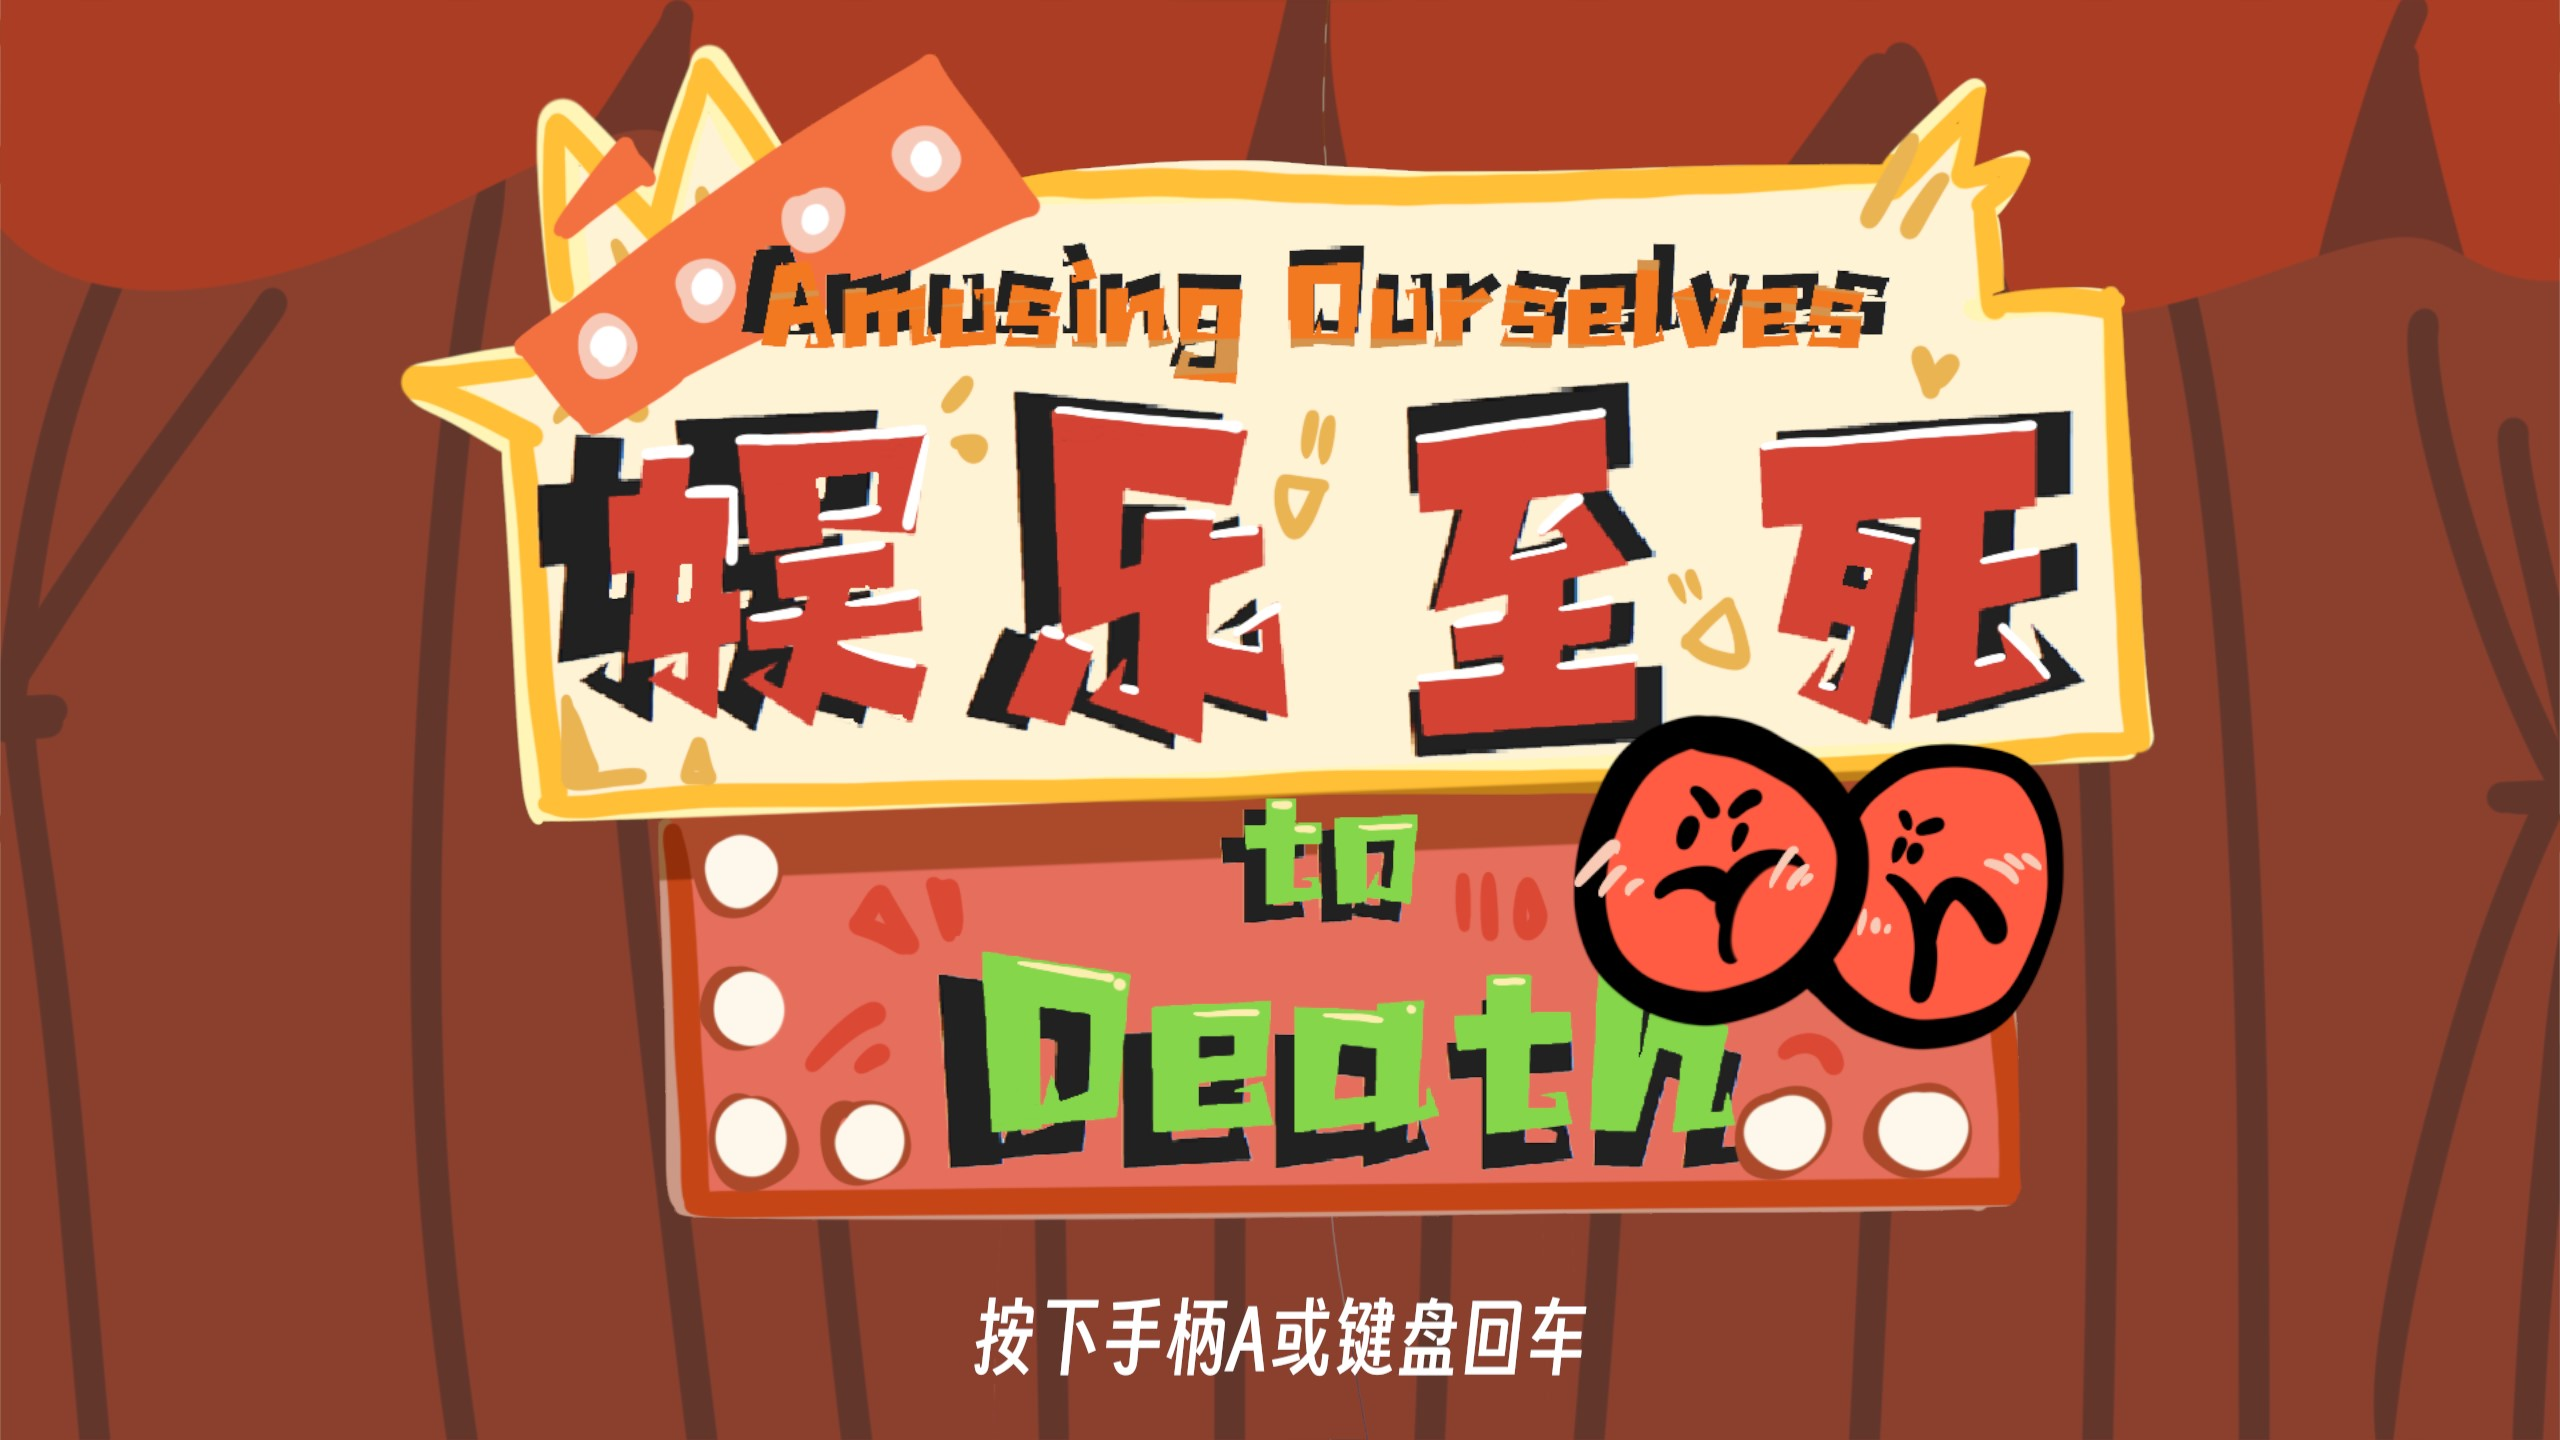
\includegraphics[width=0.8\textwidth]{Images/娱乐至死/ylzs.jpeg}
    \caption{娱乐至死\ 游戏封面}
\end{figure}

\begin{figure}[H]
\centering  %图片全局居中
\subfigure[玩家准备画面]{
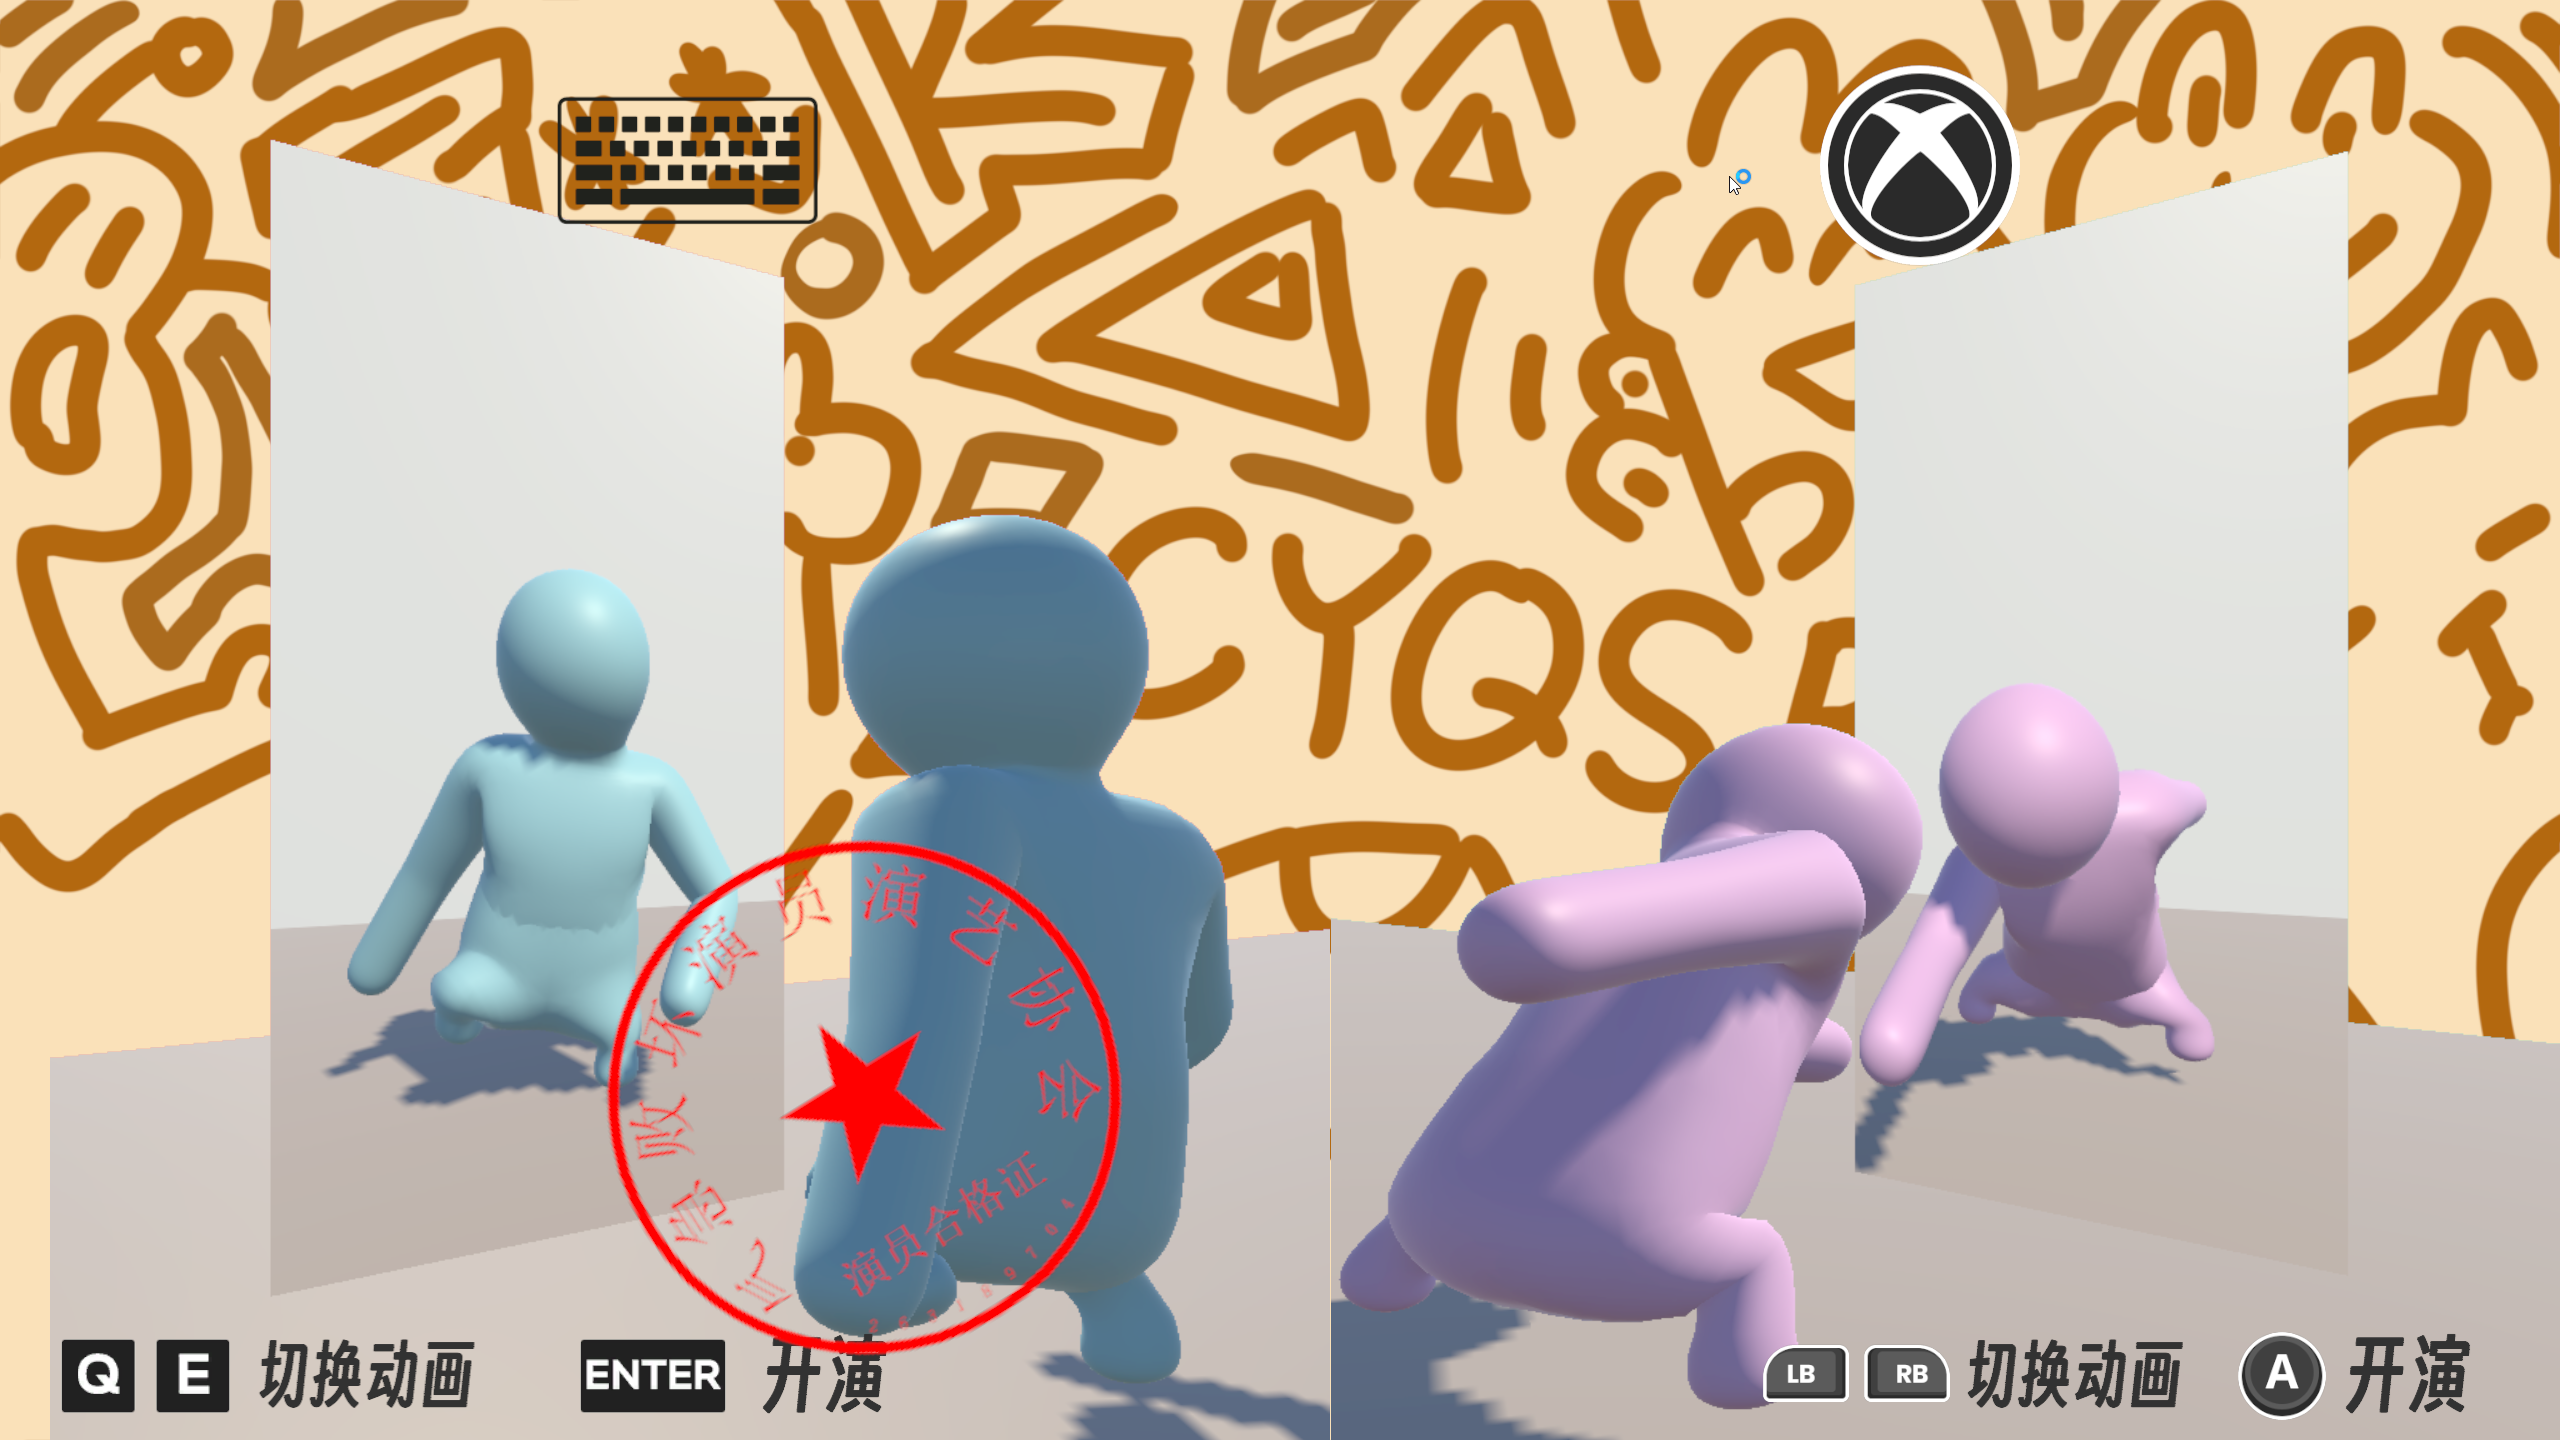
\includegraphics[width=0.45\textwidth]{Images/娱乐至死/ylzs0.png}}
\subfigure[对决画面1]{
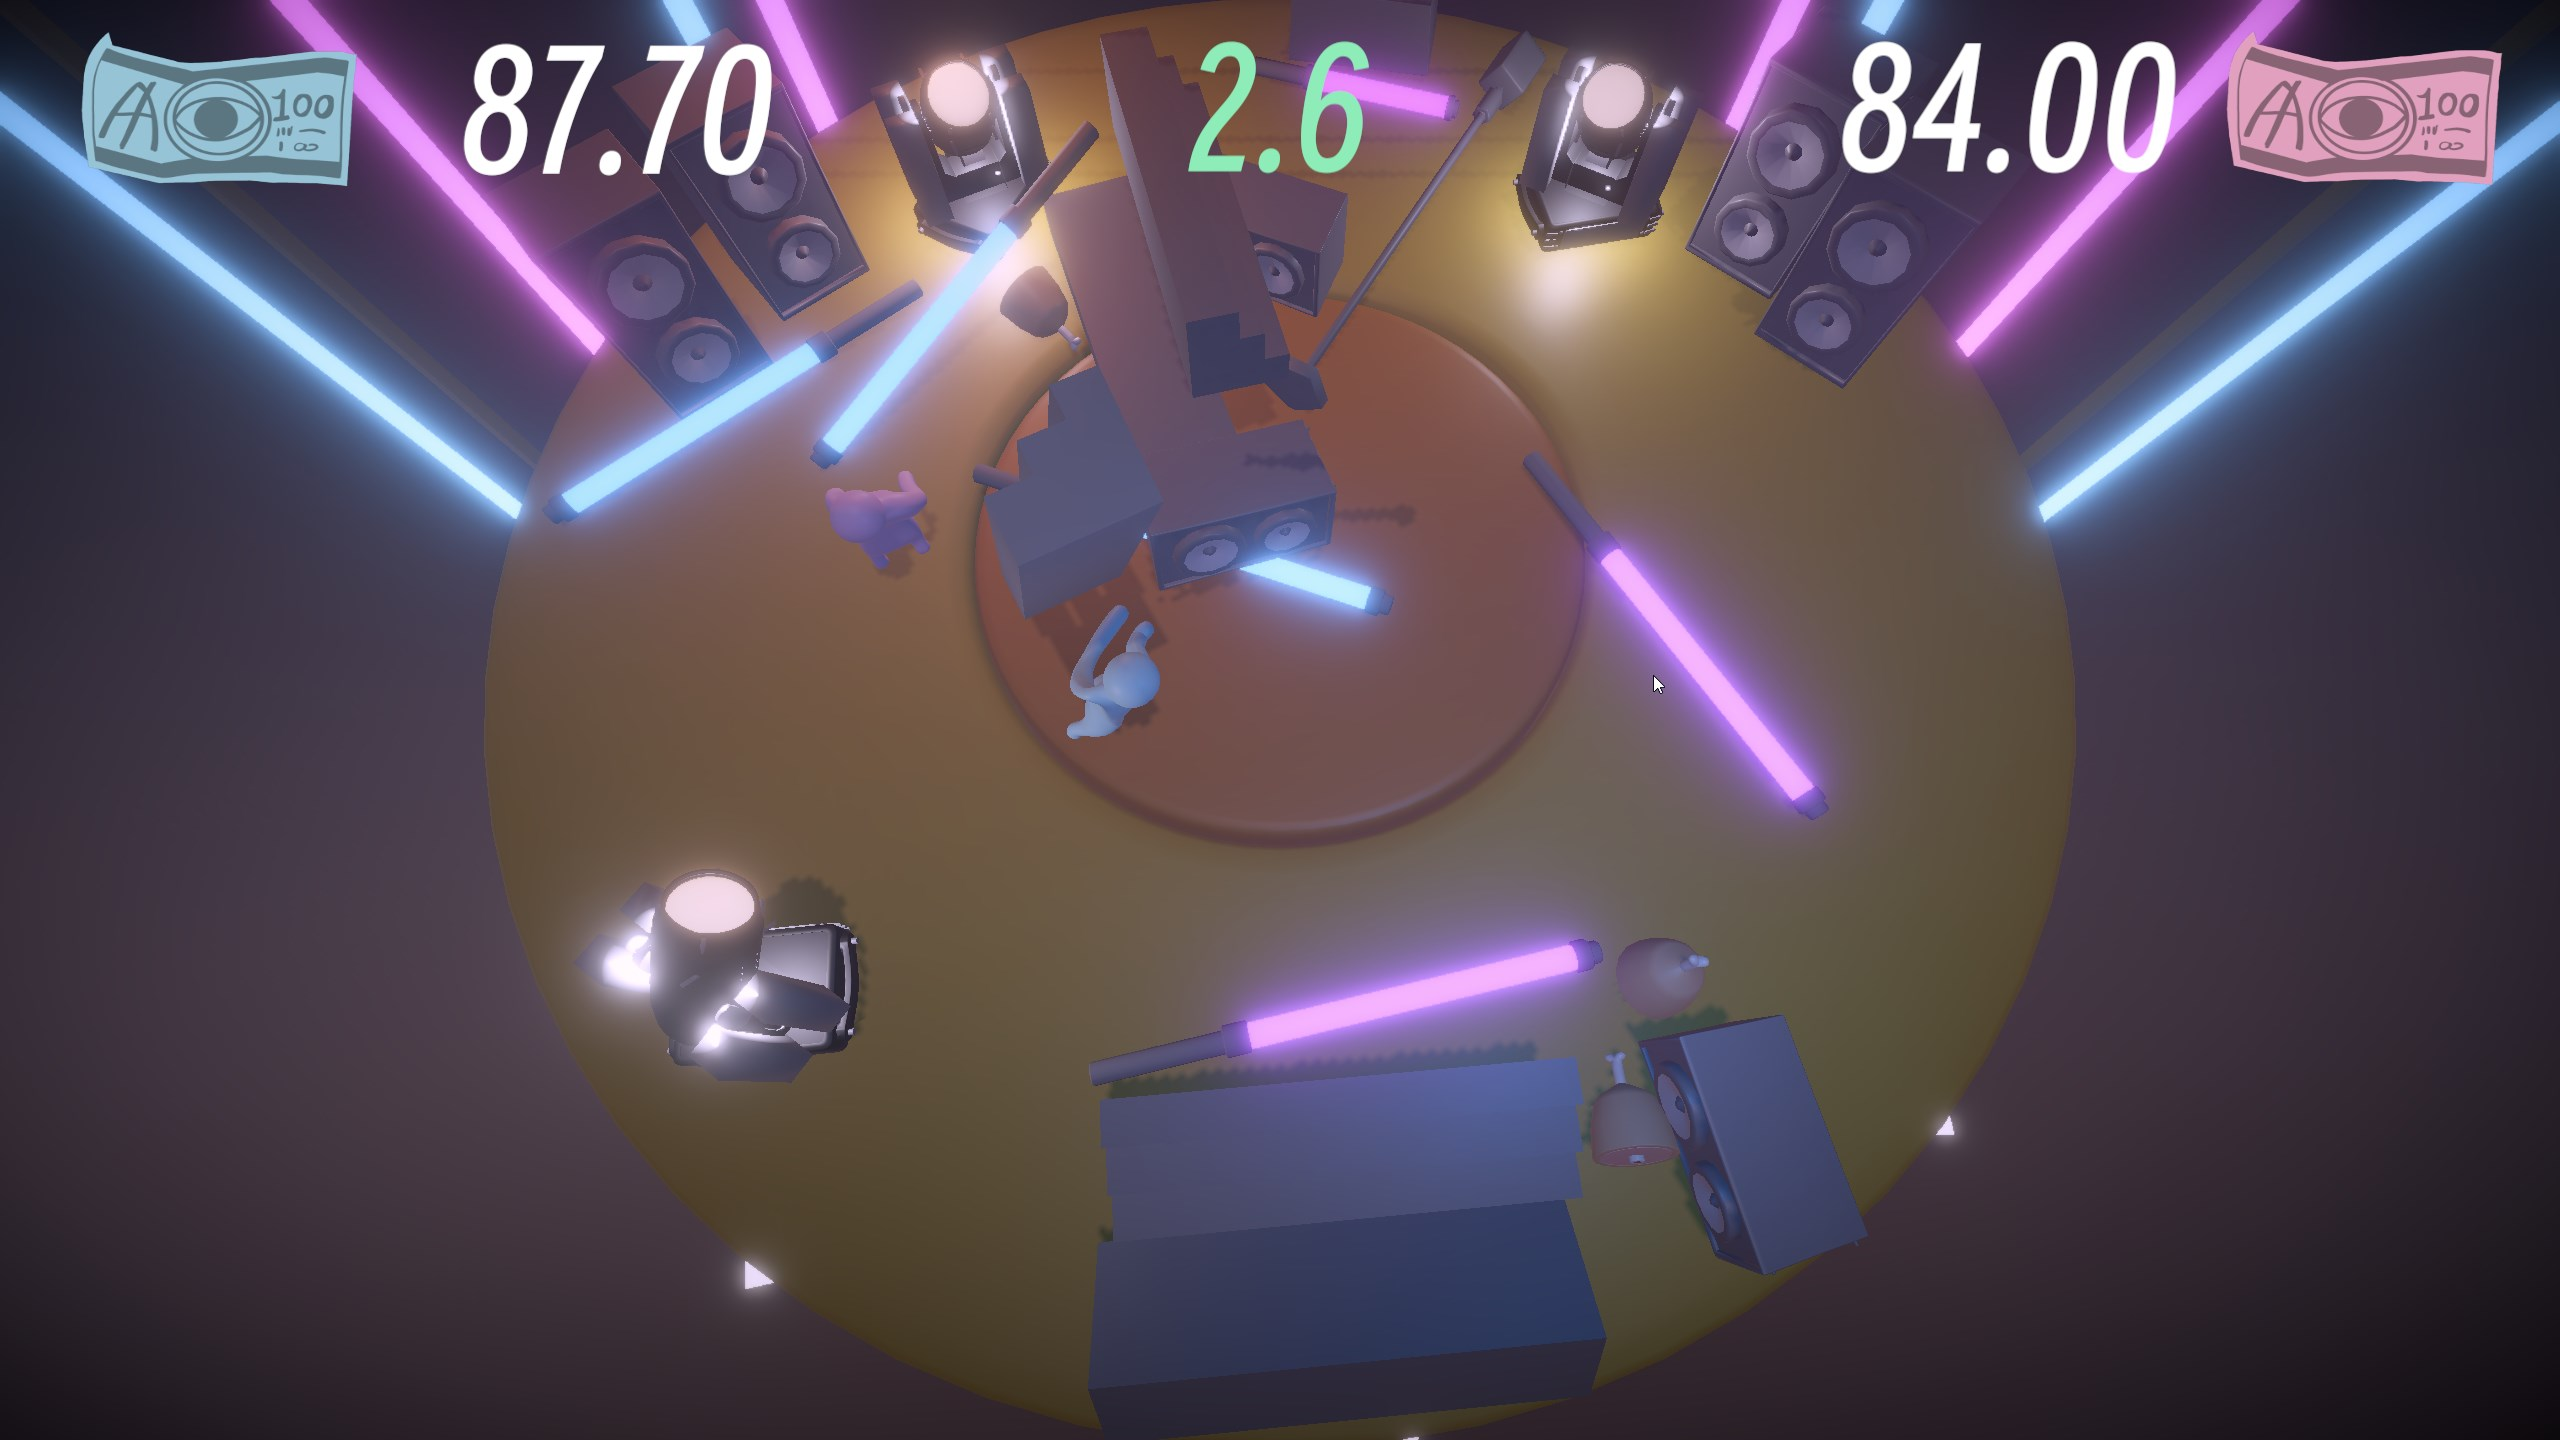
\includegraphics[width=0.45\textwidth]{Images/娱乐至死/ylzs1.jpg}}

\subfigure[对决画面2]{
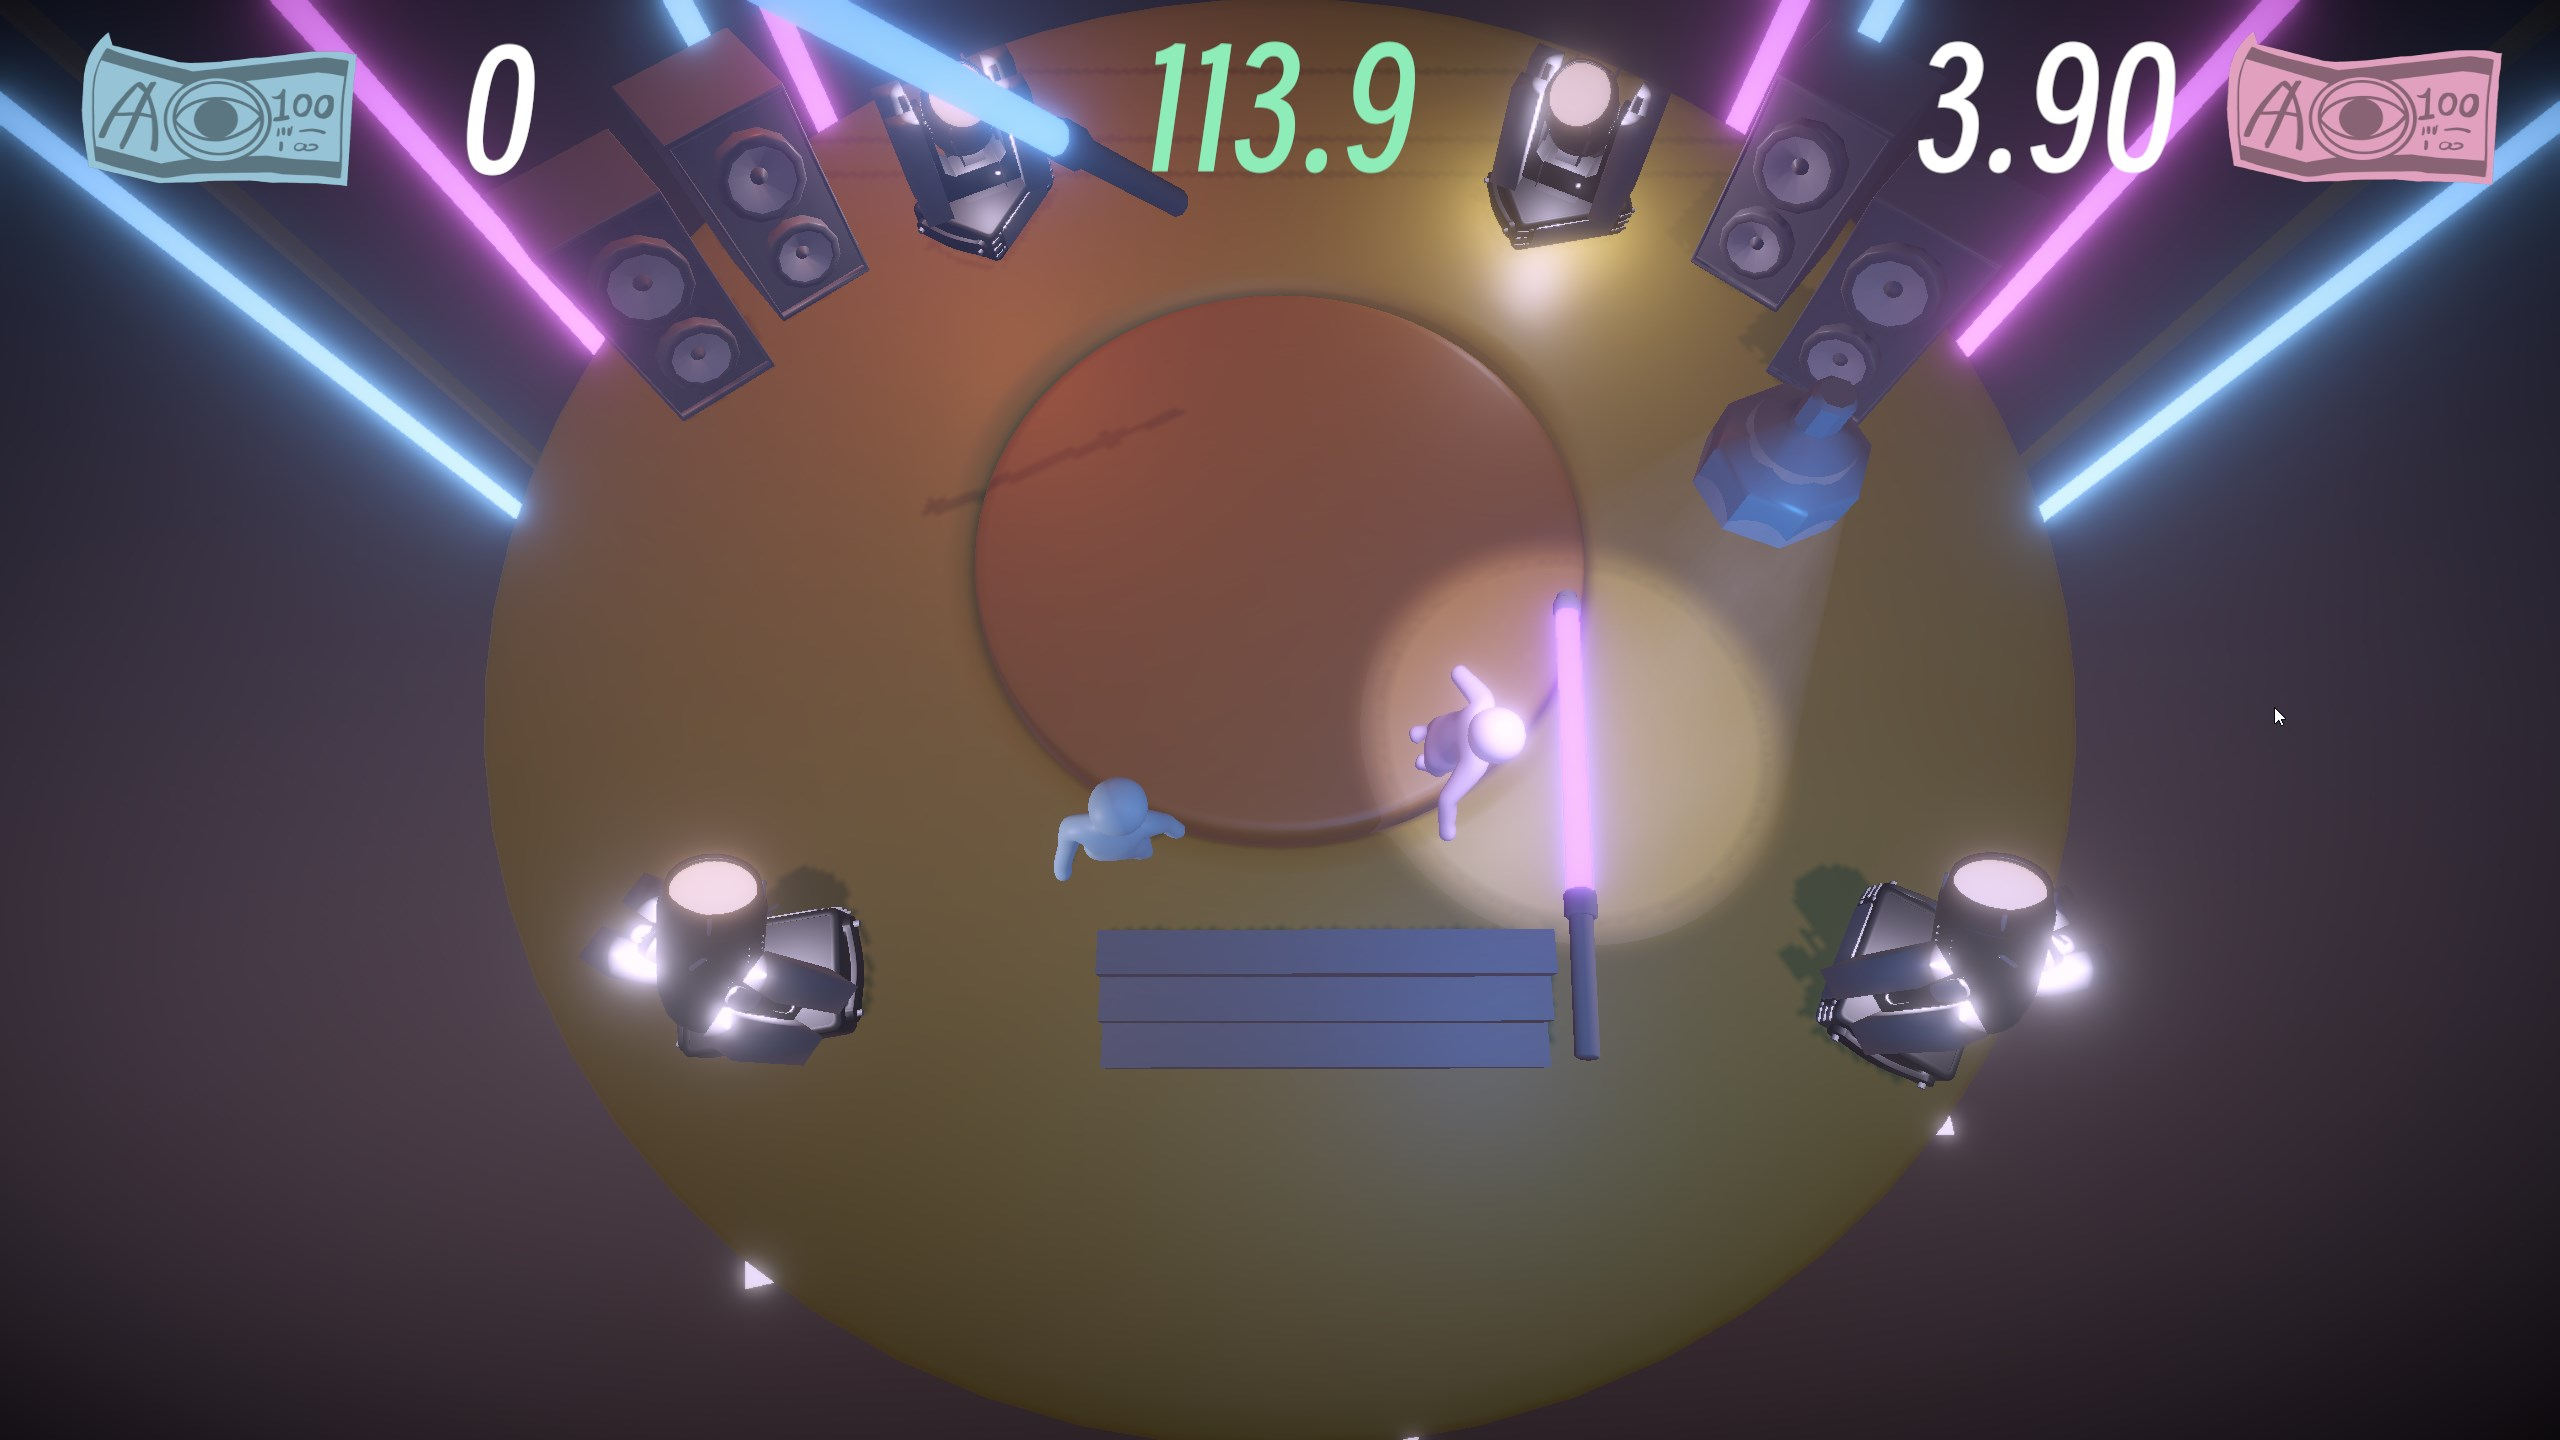
\includegraphics[width=0.45\textwidth]{Images/娱乐至死/ylzs2.jpg}}
\subfigure[结算画面]{
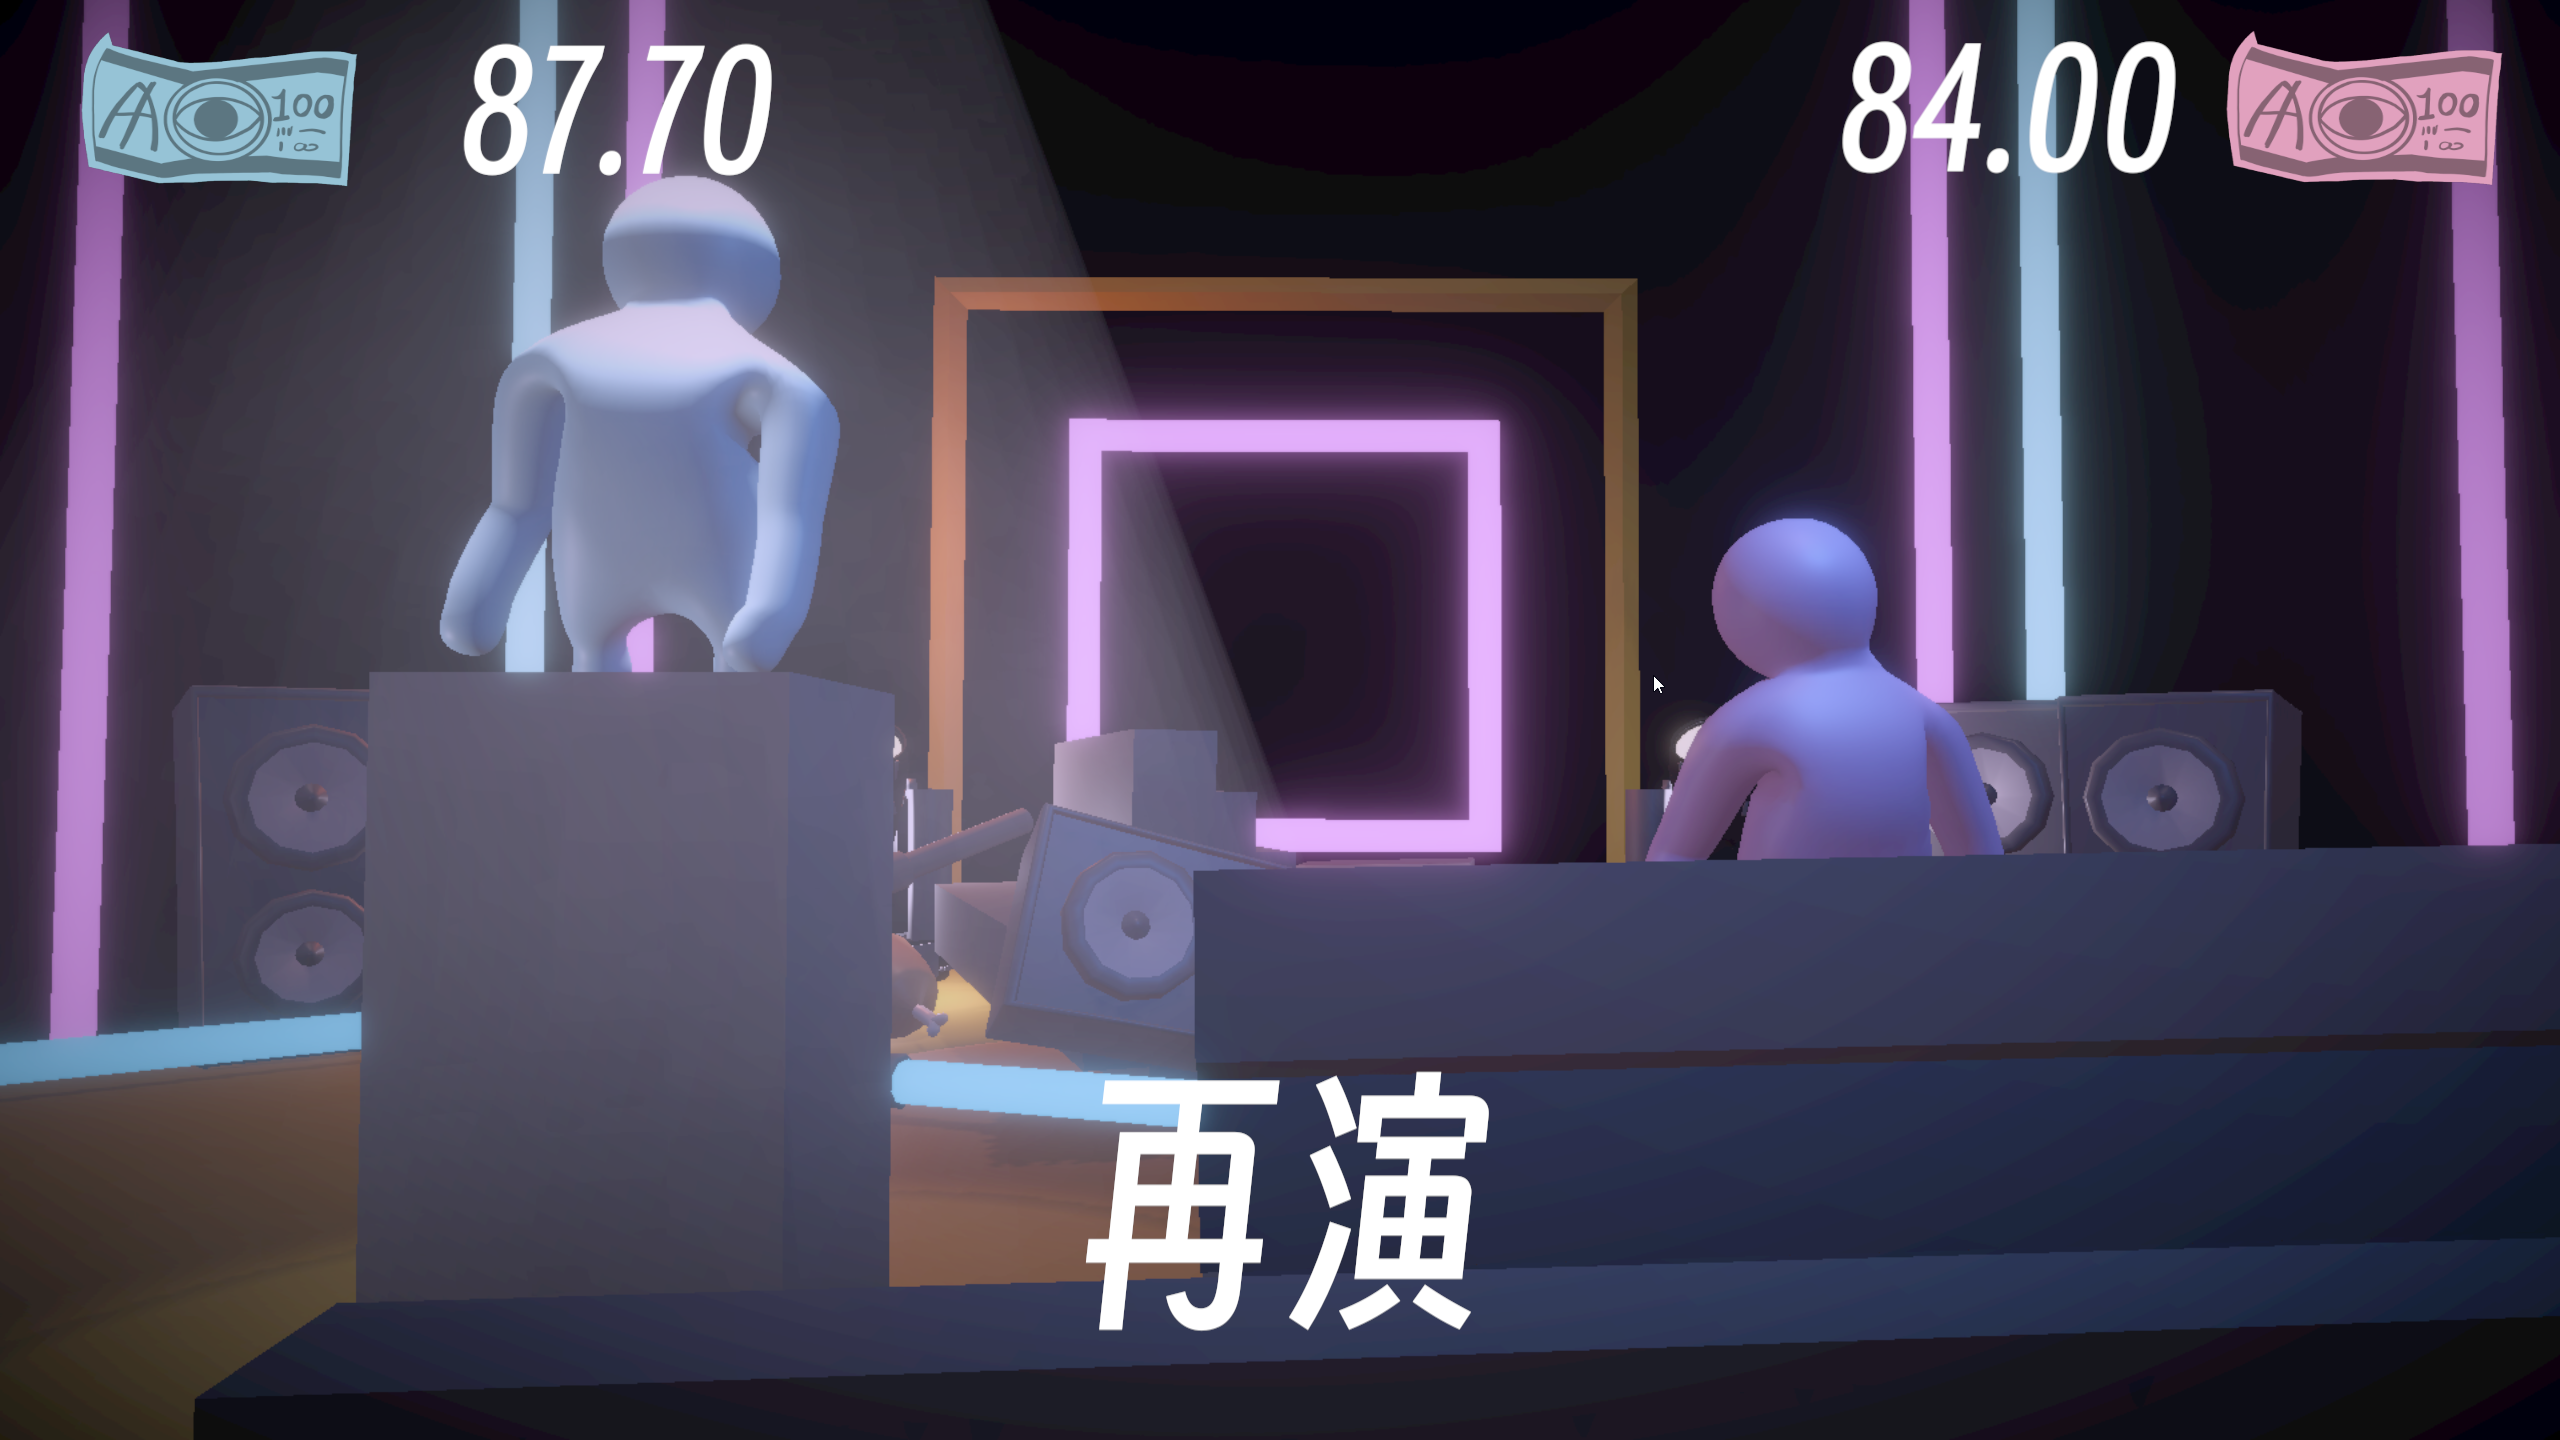
\includegraphics[width=0.45\textwidth]{Images/娱乐至死/ylzs3.png}}
\caption{娱乐至死\ 游戏画面}
\end{figure}

\section{设计思路}
游戏是命题设计,所以我们设计时着重抓住玩家的情感体验。而气急败坏其实是我们生活中很常见的体验。被最讨厌的人嘲笑、游戏大优势被翻盘、明明能做好的事情却搞砸了。气急败坏在我们看来是一种“既得利益的丢失”和“面对外界压力的无奈”。

\begin{figure}[H]
    \centering
    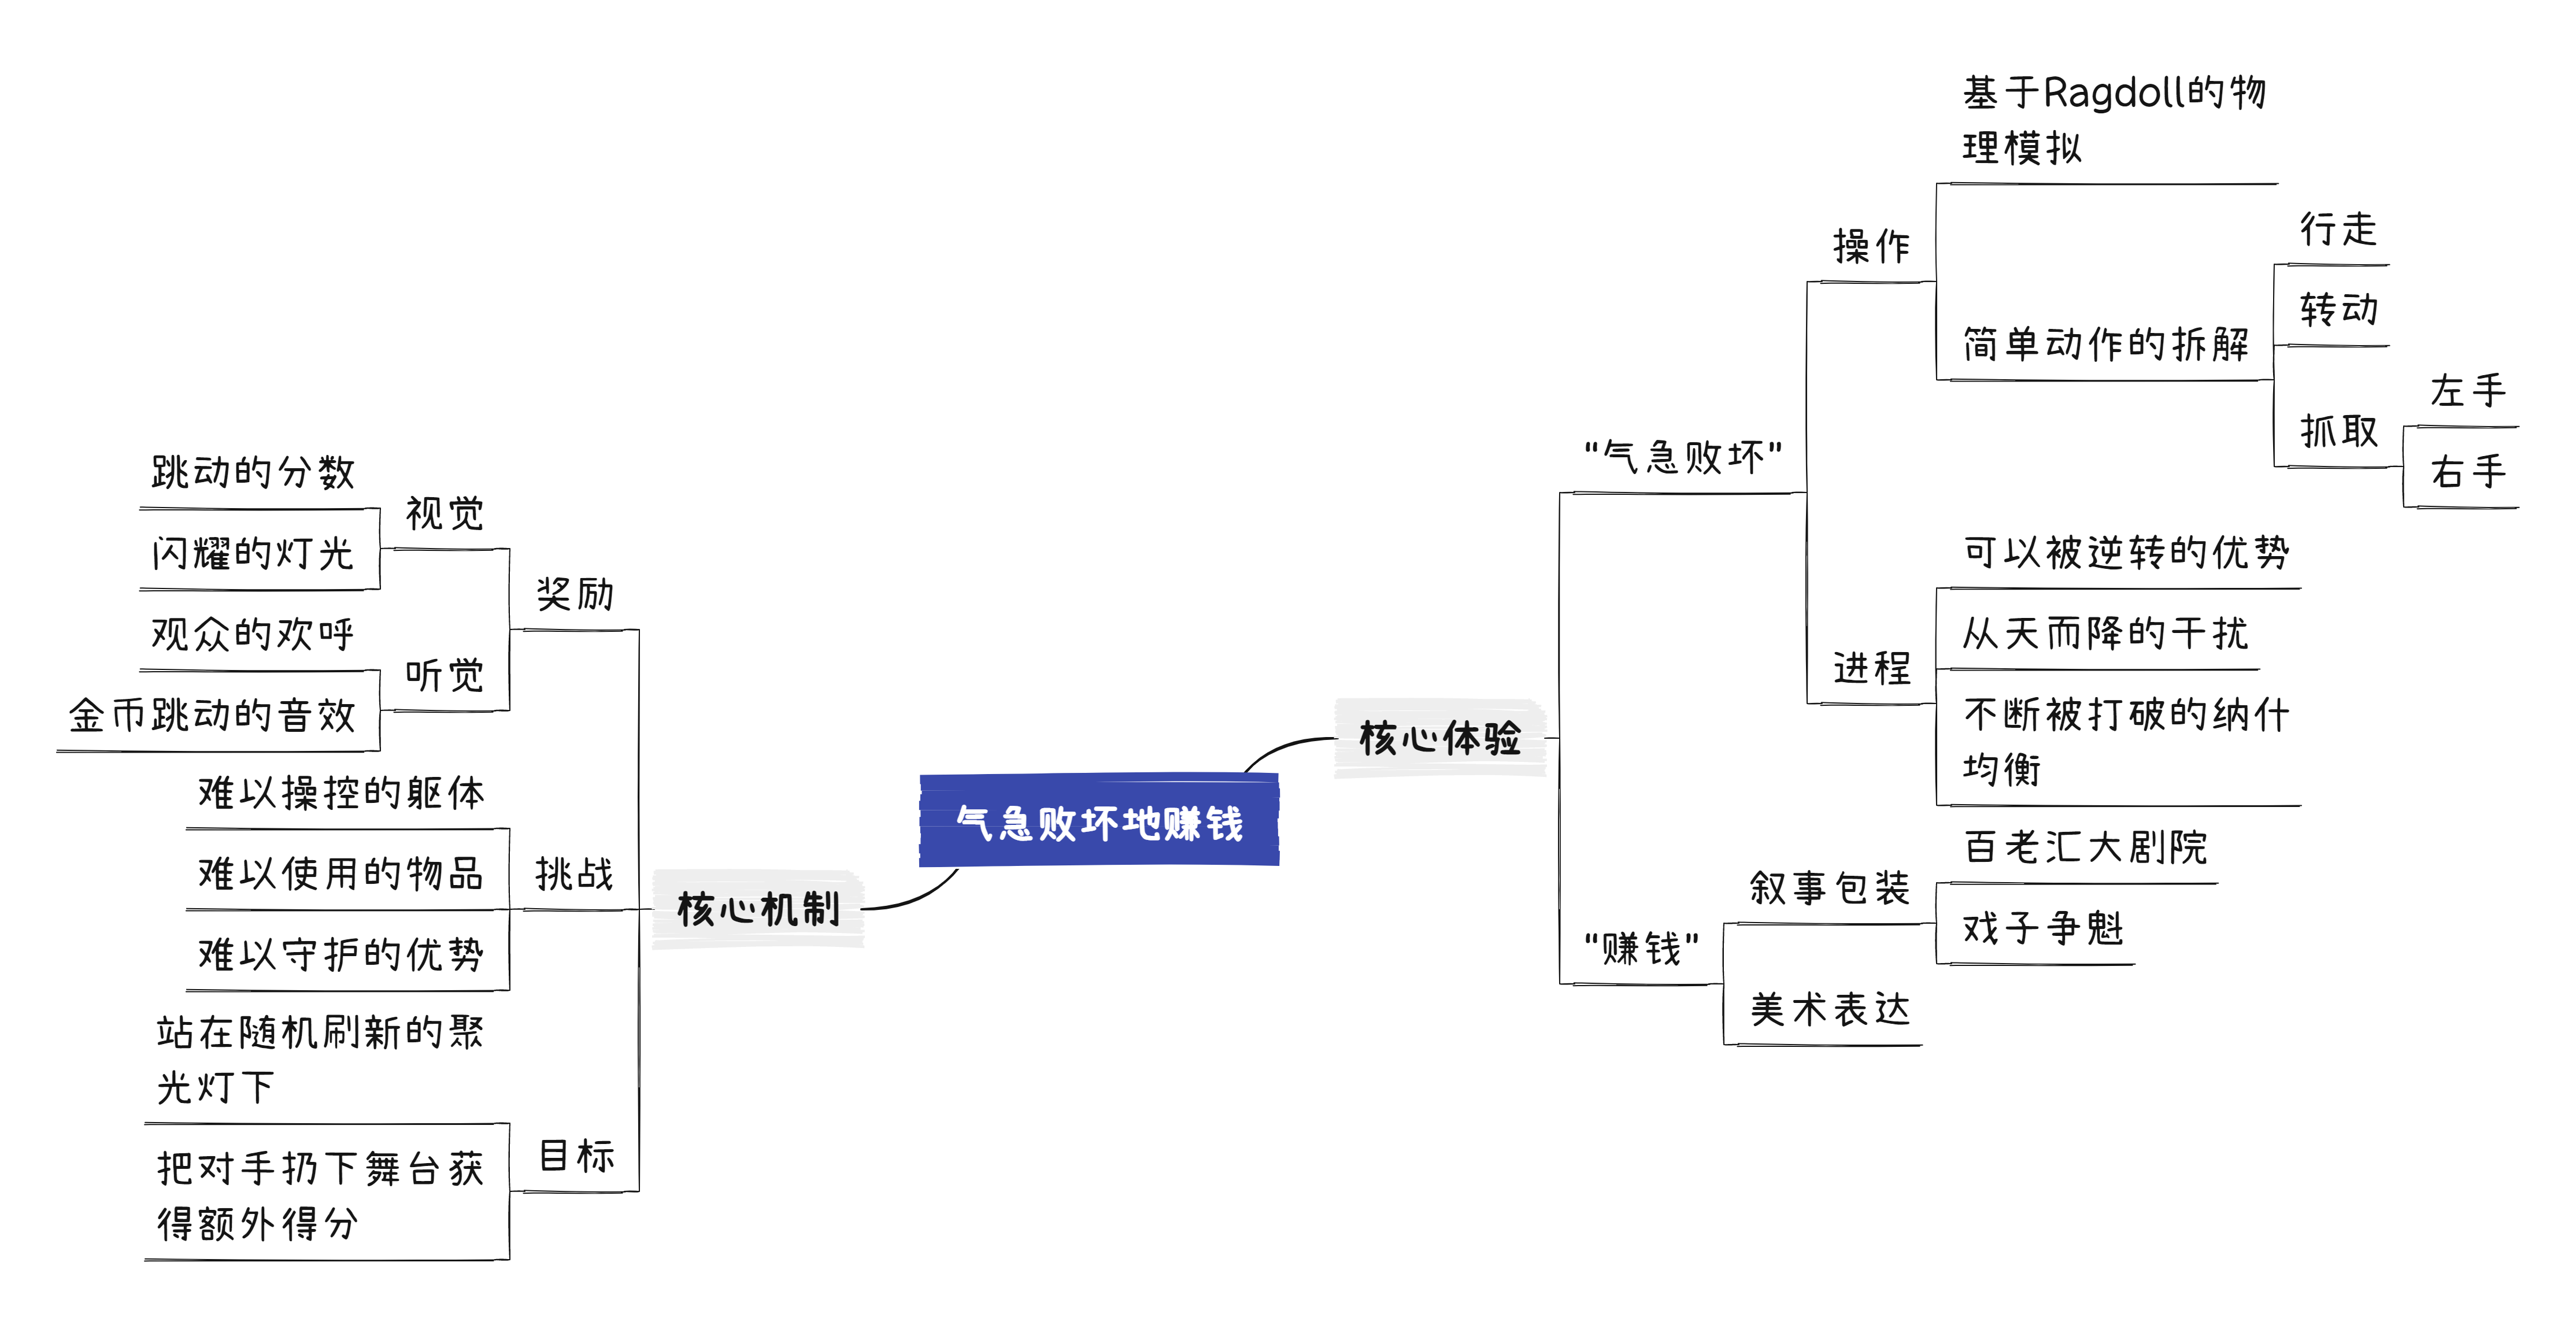
\includegraphics[width=0.9\textwidth]{Images/娱乐至死/ylzs_design.png}
    \caption{娱乐至死\ 原型设计思路}
\end{figure}

针对这两个出发点,我们在三天内做出了《娱乐至死》这款游戏。

基于Ragdoll的物理模拟的灵感来源是大名鼎鼎的《人类一败涂地》,糟糕的操作手感、难以控制的动作构成了玩家求而不得的破碎感,这种直接粉碎直觉的操控让玩家能够体会到什么是“面对外界压力的无奈”。为了缓冲这种负反馈,我们放弃了最初的PVE玩法,选择了本地双人对战,利用好友间的欢声笑语冲淡操作带来的滑稽和无奈。

建立极大的优势后再次失去也会瞬间让人崩溃则代表了“既得利益的丢失”。所以确定好游戏要努力站在聚光灯下得分的玩法后,我们加入了随机掉落的道具和掉落失分机制。高水平玩家可以通过挥舞、投掷随机掉落的道具攻击其他玩家。而玩家如果掉下舞台会给对方增加极大的分数,所以一切在聚光灯下累积的优势很可能在对手优秀的操作或自身失误后立刻瓦解。在给予优势方气急败坏的游戏体验时,也给落后方一个翻盘的可解性。不断推翻的纳什均衡使得玩家要不断在游戏里做出操作和决策。

\section{演示链接}
\begin{itemize}
    \item \textbf{试玩视频:}  \href{https://www.bilibili.com/video/BV13M411n7Dp/?vd_source=ead0ac501dfae814e19fd7d9f376d92d}{Bilibili视频}
    \item \textbf{Demo下载:}  \href{https://scyq.itch.io/amusing-ourselves}{itch.io界面} 
\end{itemize}